
\renewcommand{\EntradaBibtex}{RealidadAumentada_PrimerPrototipo_2019}
\begin{frame}{\citetitle{\EntradaBibtex} \footnotemark[1] (1)}

%\begin{frame}{Sistema de Realidad Aumentada \footnotemark}
%\begin{block}{Sistema de Realidad Aumentada \footnotemark} 
\begin{columns}
\begin{column}{0.48\textwidth}
		\begin{itemize}
		\item Detección de Codigos QR
		\item Decodificación del texto codificado en el codigo QR
		\item Sobreposición del modelo 3D dependiendo de la posición del código QR
		\end{itemize}
	\end{column}
	\begin{column}{0.52\textwidth}  
	    \begin{center}
	    	 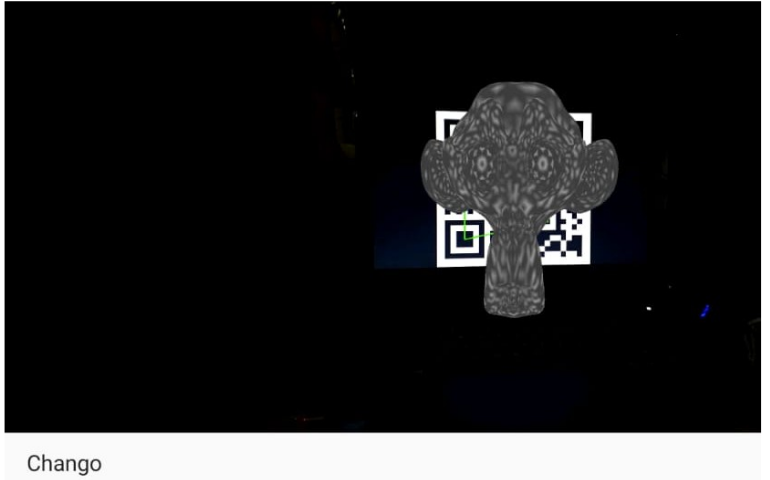
\includegraphics[width=0.95\textwidth]{Figs/SistemaAR1}
    	 \end{center}
	\end{column}
	\end{columns}
%	\end{block} 
\footnotetext[1]{\fullcite{\EntradaBibtex}}
%\footnotetext{Cárdenas Castillo Jesús Alfredo, Molina Pastrana Ana Karen, Ramos Lucio Eluis Carlo, Rodríguez Terán Linda Margarita y Vázquez Luna César Jovany.  \textbf{Visión por Computadora para Realidad Aumentada}. Universidad Politécnica de Victoria,  Informe técnico proyecto de asignatura ``Cómputo en Dispositivos Móviles'', 2019. Sin Publicar.}
%\\setcounter{footnote}{0}
\end{frame}

%Cárdenas Castillo Jesús Alfredo, Molina Pastrana Ana Karen, Ramos Lucio Eluis Carlo, Rodrı́guez Terán Linda Margarita, Vázquez Luna Cesar Jovany.
% \textbf{Visión por Computadora para Realidad Aumentada}. Universidad Politécnica de Victoria,  Informe técnico proyecto de asignatura ``Cómputo en Dispositivos Móviles'', 2019. Sin Publicar.

\begin{frame}{\citetitle{\EntradaBibtex} (2)}
%\begin{block}{Sistema de Realidad Aumentada (2)} 
\begin{columns}
\begin{column}{0.5\textwidth}
    \begin{center}
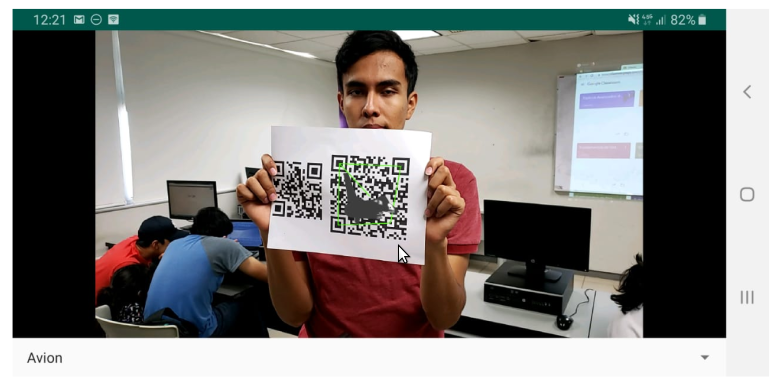
\includegraphics[width=0.98\textwidth]{Figs/SistemaAR2}\\
     \end{center}

\end{column}
\begin{column}{0.5\textwidth}  
    \begin{center}
\begin{itemize}
\end{itemize}

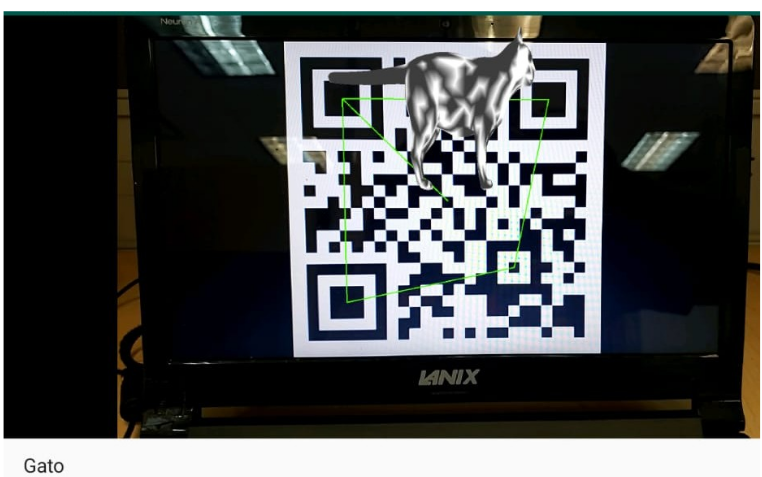
\includegraphics[width=0.98\textwidth]{Figs/SistemaAR3}\\
     \end{center}
\end{column}
\end{columns}



%\end{block} 
\end{frame}

